\documentclass[12pt]{article}
\thispagestyle{empty}
\usepackage{amsmath}
\usepackage[margin=1in]{geometry}
\usepackage{amsfonts}
\usepackage{hyperref}
\usepackage{graphicx}
\usepackage{siunitx}
\usepackage{cancel}
\usepackage{xfrac}
\usepackage{listings}

\begin{document}
	
	\begin{center}
		\par\noindent \large \textbf{Binary Arithmetic (part 1)}  [Andy Chong Sam]
	\end{center}
	
	\par\noindent In this article we'll describe the simplest forms of binary addition and subtraction. In these operations we'll deal with positive and whole numbers only.
	
	\section{Binary Addition}
	
	\begin{minipage}[t]{.5\linewidth}
			
		\par\noindent \textbf{(I)} We first establish some basic binary results. The decimal equivalent is listed on the right:
		\begin{flalign*}
			\textbf{Binary} \;\;\;\;\;\; \textbf{Decimal} \\
			0 + 0 = 0 \;\;\;\;\;\; 0 + 0 = 0 \\
			0 + 1 = 1 \;\;\;\;\;\; 0 + 1 = 1 \\
			1 + 1 = 10 \;\;\;\;\;\;1+1=2 \\
			10 + 1 = 11\;\;\;\;\;\;2+1=3
		\end{flalign*}
		\par\noindent  Just like with regular decimal addition, we stack both binary numbers and add the columns. If we need to perform a \(1+1\) or \(10+1\), a \(1\) is sent to the carry for the next column.
		\newline
		\par\noindent \textbf{(II)} Let's see a simple example, the decimal operation 2 + 3 = 5. We know that 2 in binary is \(10\) and 3 in binary is \(11\), so:
		\begin{center}
		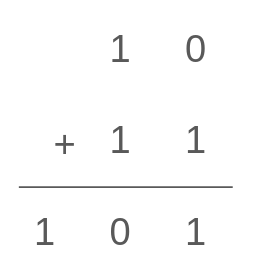
\includegraphics[width=3cm]{bin-add-1.png}
		\end{center}
		\par\noindent On the first column we have \(0+1=1\), next we have have \(1+1=10\). We can confirm that this result is 5 since \((1)(2)^0 + (1)(2)^2 = 5\).
	\end{minipage}
	\hspace{0.45cm}
	\begin{minipage}[t]{.5\linewidth} 
	\par\noindent \textbf{(III)} Let's see what happens with \(14 + 5 = 9\). In binary \(14\) is \(1110\) and \(5\) is \(101\):
	\begin{center}
		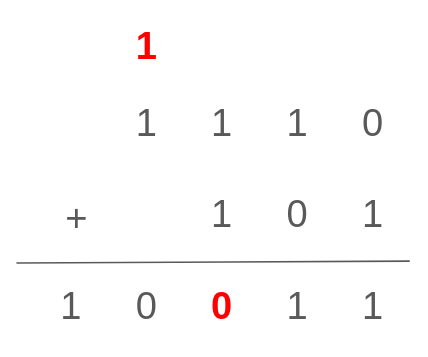
\includegraphics[width=5cm]{bin-add-2.png}
	\end{center}
	\par\noindent So we can follow our rules fairly well until we get to the third column where we need to do \(1+1=10\). In this case we will record the \(0\) and the 1 moves to the carry position of the next column. The operation on the last column thus becomes \(1+1=10\).
	\newline
	\par\noindent \textbf{(IV)} Now let's try \(14 + 15\). In binary, 14 is \(1110\) and 15 is \(1111\):
		\begin{center}
		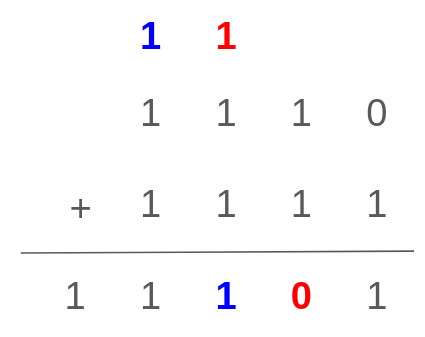
\includegraphics[width=5cm]{bin-add-3.png}
	\end{center}
	
	\par\noindent On the second column we will record the 0 but move the 1 to the third column's carry position. On the third column we will have to calculate \(1+1+1\). In binary, \(1+1 = 10\) and \(10+1=11\). We record the 1 and move a 1 to the fourth column's carry. On the last column we will again compute \(1+1+1\).
	
	\end{minipage}
	\section{Binary Subtraction}
		\begin{minipage}[t]{.5\linewidth}
					\par\noindent \textbf{(I)} Just like with addition, we'll list out some basic operations first.
			\begin{flalign*}
				\textbf{Binary} \;\;\;\;\;\; \textbf{Decimal} \\
				0 - 0 = 0 \;\;\;\;\;\; 0 - 0 = 0 \\
					1 - 1 = 0 \;\;\;\;\;\;1 - 1 =0 \\
				1 - 0 = 1 \;\;\;\;\;\; 1 - 0 = 1 \\
			\end{flalign*}
			\par\noindent \textbf{(II)} Let's examine the case of \(3-1=2\). In binary 3 is \(11\). This is a simple example without the need to borrow:
			\begin{center}
				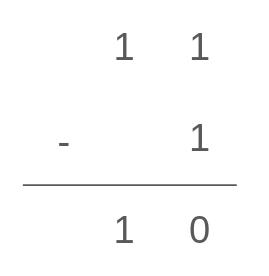
\includegraphics[width=3cm]{bin-sub-1.png}
			\end{center}
			\par\noindent This is consistent with our expectations as 2 in binary is \(10\).
			\newline
			\par\noindent \textbf{(III)} If we encounter a \(0-1\), we will need to borrow two 1's from some column towards the left. Let's consider the case of \(14-3=11\). In binary 14 is \(1110\). From the start, we need to borrow from the next column:
			\begin{center}
			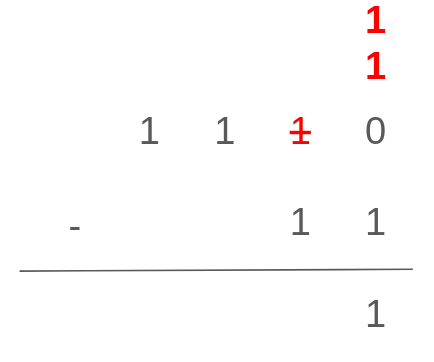
\includegraphics[width=5.5cm]{bin-sub-2.png}
			\end{center}			
		\end{minipage}
		\hspace{0.45cm}
	\begin{minipage}[t]{.5\linewidth} 
					\par\noindent Since the second column is now zero, we proceed to borrow from the third column:
		\begin{center}
			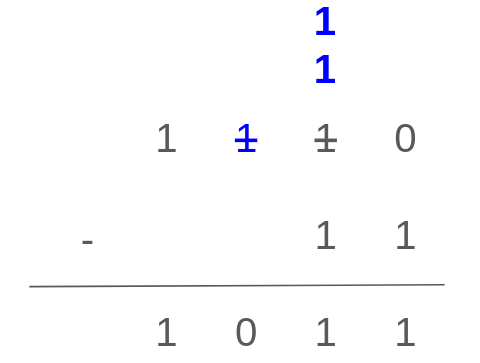
\includegraphics[width=5.5cm]{bin-sub-3.png}
		\end{center}
	
	\par\noindent \textbf{(IV)} Let's examine one final example, \(17-15=2\). In binary, \(17\) is \(10001\) and \(15\) is \(1111\).
			\begin{center}
		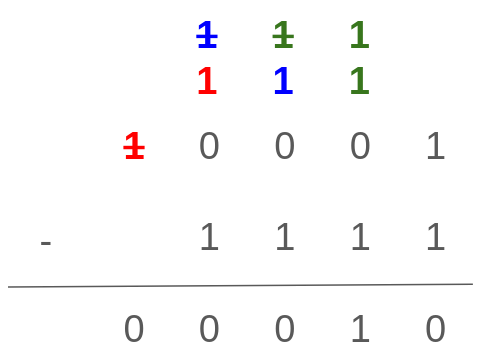
\includegraphics[width=5.5cm]{bin-sub-4.png}
	\end{center}

	\par\noindent We are able to calculate the first column, but since the second, third, and fourth columns are zero's we can only borrow from the last column. So:
	
	\begin{itemize}
		\item The fifth column loses a 1, and the fourth gains two 1's.
		\item The fourth column loses a 1, and the third column gains two 1's.
		\item The third column loses a 1, and the second column gains two 1's.
	\end{itemize}
		\end{minipage}
	\newline
	\par\noindent \textbf{(V)} To conclude, let's discuss why lending a 1 results in two 1's on the right. If the right most column is \(n=0\), then the decimal value of a \(1\) on column n is \(2^n\). On the example above, 17 has a 1 on column n=4 with a decimal value of \(2^4 = 16\). If we transfer this amount to column n=3, the transferred amount can be represented with two 1's, each with a decimal value of \(2^3=8\).
	
\end{document}